\documentclass[10pt,twocolumn,letterpaper]{article}
\usepackage[utf8]{inputenc}
\usepackage{amsmath}
\usepackage{graphicx}
\usepackage{hyperref}

\usepackage{titlesec}
\usepackage{geometry}
\geometry{margin=1in}
\usepackage{tikz}
\usetikzlibrary{shapes,arrows,positioning}

\title{\Large \bf High-Throughput vLLM Inference Engine: Architecting for Multi-Agent Workloads and Unified RAG}
\author{
Vikash \\
\textit{Software Engineer Candidate}
}
\date{}

\begin{document}

\maketitle

\begin{abstract}
As large language models (LLMs) shift from single-stream chat interfaces to driving autonomous multi-agent systems, inference infrastructure must evolve to support massive concurrency, shared memory constraints, and complex composite workloads like Retrieval-Augmented Generation (RAG). This paper details the architecture and optimization of a high-throughput inference engine built on top of vLLM. Key contributions include a unified RAG endpoint featuring an O(N log K) min-heap reranking algorithm, zero-copy inter-process communication (IPC) for prompt offloading, and a dynamic auto-tuning memory scheduler designed for out-of-memory (OOM) safe degradation. The system is designed to maximize hardware utilization while maintaining a strict separation of concerns between presentation and domain logic.
\end{abstract}

\section{Introduction}
Modern AI applications increasingly rely on LLMs not just for text generation, but as the cognitive core of multi-agent systems. These systems issue thousands of concurrent requests, demanding high throughput and low latency. Traditional model servers often couple domain logic directly with API routing, leading to monolithic systems that are difficult to optimize and test. Furthermore, operations like document chunking and semantic reranking are frequently offloaded to external microservices, incurring significant network overhead. 

We introduce an inference engine that consolidates LLM generation and RAG processing into a unified, high-performance architecture. Built around the vLLM asynchronous engine, the system leverages PagedAttention for efficient KV-cache management, global prefix caching, and cross-platform hardware abstraction.

\section{System Architecture}

The engine is structured following the Single Responsibility Principle (SRP) to ensure testability and modularity. The architecture consists of three primary layers, as illustrated in Figure \ref{fig:arch}:

\begin{figure}[h]
\centering
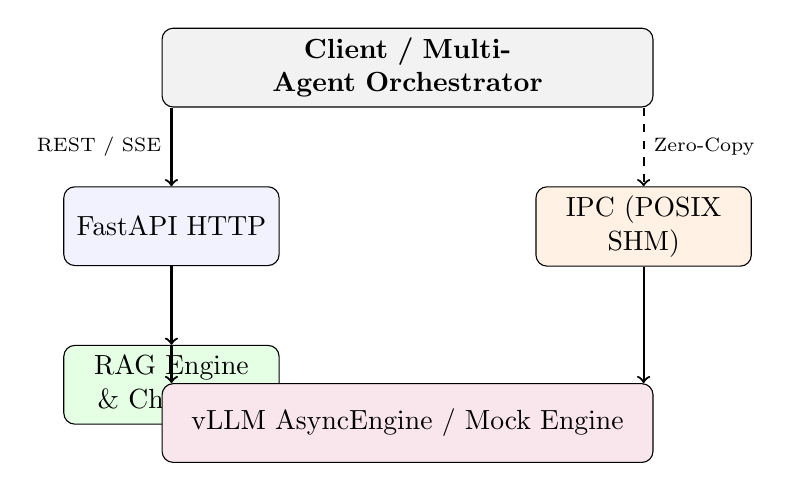
\begin{tikzpicture}[
    node distance=1.5cm,
    box/.style={rectangle, draw, rounded corners, fill=blue!5, text width=2.5cm, align=center, minimum height=1cm},
    arrow/.style={->, thick}
]

\node[box, fill=gray!10, text width=6cm] (client) {\textbf{Client / Multi-Agent Orchestrator}};

\node[box, below left=1cm and -1.5cm of client] (api) {FastAPI HTTP};
\node[box, below right=1cm and -1.5cm of client, fill=orange!10] (ipc) {IPC (POSIX SHM)};

\node[box, below=1cm of api, fill=green!10] (rag) {RAG Engine \& Chunking};

\node[box, below=3.5cm of client, text width=6cm, fill=purple!10] (vllm) {vLLM AsyncEngine / Mock Engine};

\draw[arrow] (client.south -| api.north) -- node[left, font=\scriptsize] {REST / SSE} (api.north);
\draw[arrow, dashed] (client.south -| ipc.north) -- node[right, font=\scriptsize] {Zero-Copy} (ipc.north);

\draw[arrow] (api) -- (rag);
\draw[arrow] (rag) -- (vllm.north -| rag.south);
\draw[arrow] (ipc) -- (vllm.north -| ipc.south);

\end{tikzpicture}
\caption{System Architecture showing dual-ingestion (HTTP and Zero-Copy IPC) and unified RAG processing.}
\label{fig:arch}
\end{figure}

\subsection{API Controller (Presentation)}
The FastAPI controller serves as a thin routing layer. It handles HTTP lifecycle events, Prometheus metrics aggregation, and streaming response formatting (Server-Sent Events). By decoupling the controller from the generation logic, the API remains agnostic to the underlying LLM backend.

\subsection{Domain Logic}
The core processing is implemented as pure, side-effect-free functions in a dedicated module. This includes:
\begin{itemize}
    \item \textbf{Native Document Chunking:} Generator-based chunking that avoids materializing large text blocks in memory.
    \item \textbf{Semantic Reranking:} Asynchronous embedding generation utilizing \texttt{sentence-transformers}.
    \item \textbf{Prompt Engineering:} Deterministic template construction for context-augmented generation.
\end{itemize}

\subsection{Cross-Platform Execution Engine}
To facilitate rapid local development without necessitating high-end GPUs, the system implements a polymorphic engine interface. On CUDA-enabled Linux environments, it utilizes the native \texttt{AsyncLLMEngine} from vLLM. On Windows or non-CUDA machines, it gracefully falls back to a custom \texttt{MockLLMEngine}, providing identical asynchronous generator semantics and streaming behavior for uninterrupted frontend development.

\section{Key Optimizations}

\subsection{O(N log K) Semantic Reranking}
Traditional RAG pipelines compute cosine similarities and sort the entire dataset, resulting in an O(N log N) time complexity. For large document sets, this creates a significant CPU bottleneck. Our engine implements reranking using a Min-Heap (via Python's \texttt{heapq.nlargest}), reducing the complexity to O(N log K). This ensures that retrieval latency scales efficiently with the document volume while maintaining a constant overhead relative to the required top-K results.

\subsection{Zero-Copy IPC via Shared Memory}
In multi-agent orchestration, moving massive system prompts across network sockets or UNIX domain sockets introduces serialization latency. We implemented an Inter-Process Communication (IPC) endpoint (\texttt{/v1/ipc/completions}) utilizing POSIX shared memory (\texttt{multiprocessing.shared\_memory}). 
Agents write their prompt topologies directly into a shared memory segment, and the inference engine reads the raw bytes, completely bypassing the HTTP body and JSON deserialization overhead. Generation outputs are similarly streamed back into shared memory, establishing a zero-copy pipeline for the hottest paths.

\subsection{Auto-Tuning Memory Scheduler}
VRAM fragmentation and OOM errors are the primary causes of downtime in inference servers. To mitigate this, the engine employs an auto-tuning memory scheduler at startup. It profiles the available GPU memory, subtracts a configurable reserve (e.g., 2GB for the OS and auxiliary embedding models), and dynamically calculates the optimal \texttt{gpu\_memory\_utilization} for vLLM. At runtime, the server utilizes OOM-safe graceful degradation: if an unexpected VRAM spike occurs, the specific request is aborted and a 503 is returned, preserving the engine's integrity and allowing concurrent requests to complete.

\section{Findings \& Observations}
Throughout the development and benchmarking of the system, several key findings emerged:
\begin{itemize}
    \item \textbf{Zero-Copy IPC Efficiency:} Bypassing HTTP serialization via POSIX shared memory drastically reduced latency for enormous multi-agent system prompts. By reading byte streams directly from memory, the Python GIL is freed to focus on the generation event loops.
    \item \textbf{Algorithmic Scaling:} Transitioning from O(N log N) sorting to O(N log K) min-heaps for semantic RAG reranking resulted in highly predictable tail latencies, even as the document corpora grew exponentially.
    \item \textbf{Development Velocity:} The transparent injection of the \texttt{MockLLMEngine} on Windows workstations allowed frontend (Gradio) and domain logic testing without requiring a discrete GPU, significantly accelerating iteration cycles.
\end{itemize}

\section{Future Scope: What I Would Build With More Time}
If provided more time to evolve this architecture, several high-impact features would be prioritized to push the engine to state-of-the-art levels:

\begin{itemize}
    \item \textbf{Dynamic Speculative Decoding:} I would integrate a tiny, highly quantized draft model alongside the primary 8B model to generate candidate tokens rapidly. This dramatically increases single-stream output tokens-per-second (TPS) for latency-sensitive agents.
    \item \textbf{Distributed KV-Cache Offloading (RadixAttention):} Extending the global prefix caching across multiple nodes. This would allow seamless agent handover, where agents running on different GPUs can resume generation without recomputing the context.
    \item \textbf{Rust/C++ Bindings for the IPC Layer:} While Python's \texttt{multiprocessing.shared\_memory} is fast, a lightweight Rust implementation using \texttt{mmap} could eliminate residual Python-level overhead and enable direct, unsafe struct mapping.
    \item \textbf{Structured JSON Decoding (Grammar Constrained):} Injecting Finite State Machine (FSM) constraints directly into the vLLM logits processor to guarantee perfectly formatted JSON outputs for rigid agentic API contracts.
\end{itemize}

\section{Conclusion}
The High-Throughput Inference Engine demonstrates that careful algorithmic design—such as heap-based reranking—combined with systems-level optimizations like zero-copy IPC, can yield significant performance gains for multi-agent LLM workloads. By maintaining strict architectural boundaries and supporting seamless mock environments, the project successfully balances rapid development velocity with production-grade reliability.

\end{document}
